\chapter{Controlador de corriente} \chapterlabel{Informe/4-ControladorCorriente} \label{cap:ControladorCorriente}

En este capítulo se diseña y modela el circuito encargado de controlar la corriente que circula por el electroimán. Como se vio en el capítulo anterior, el sistema trabaja con corrientes elevadas por lo que se implementan estrategias de conmutación para reducir las pérdidas de energía. Para ello se utiliza una topología de puente H con cuatro MOSFET y un \textsl{driver} que los controla. Además, se detallan los criterios tenidos en cuenta al momento de  elegir  y dimensionar todos los componentes que intervienen para lograr el correcto funcionamiento del controlador de corriente. Por último, se obtiene su función transferencia  para ser utilizada en el diseño del compensador.

\section{Descripción general}\label{sec_descripcion-general}

Para controlar la posición es necesario modificar la fuerza que ejerce el electroimán sobre la pieza móvil. Como se analizó en el capítulo \ref{cap:CaracterizacionElectroiman}, dicha fuerza esta determinada por la ecuación \ref{eq_fuerza_magnetica}, que se repite a continuación. 

\begin{equation*}
	\abs{F_{m}}=\frac{i^{2}*N^{2}*\mu_{o}*A}{4*Y_{g}^{2}}
\end{equation*}

En ella se ve que la fuerza magnética depende de la corriente del bobinado. Por lo tanto, se propone implementar un controlador de corriente que permita regular esta fuerza a partir de una tensión de entrada de referencia correspondiente al valor deseado. De forma tal que, al variar dicha tensión, se logre ajustar la fuerza ejercida.

\subsection{Comportamiento eléctrico del electroimán}\label{sec_comportamiento-electrico-electroiman}

Como se analizó en el capítulo \ref{cap:CaracterizacionElectroiman}, el electroimán puede ser modelado como una inductancia que varía con la distancia de entrehierro ($Y_g$) y una resistencia serie ($R_L$). Es decir, como un circuito RL serie cuya relación entre corriente de salida y tensión de entrada (admitancia) es:

\begin{equation} \label{eq_corriente}
	\frac{I_L}{V_L}(s)=\frac{1}{s*L_{(Y_g)}+R_L}
\end{equation}

Al aplicar la transformada inversa de Laplace a la expresión  \ref{eq_corriente}, se obtiene la respuesta temporal de la corriente ante un escalón de tensión en la entrada con amplitud $v_L$, considerando corriente inicial $I_o$ y constante de tiempo $\tau=\frac{L_{(Y_g)}}{R_L}$.

\begin{equation} \label{eq_corriente_temporal_cond_iniciales}
	i_L(t)=\frac{v_L}{R_L} + (I_o-\frac{v_L}{R_L})*e^{-\frac{t}{\tau}}
\end{equation}

En la expresión \ref{eq_corriente_temporal_cond_iniciales} se puede observar que la respuesta al escalón está compuesta por dos partes: un término con una exponencial negativa correspondiente al transitorio, y un término constante correspondiente al valor en régimen permanente $\frac{v_L}{R_L}$. El primero es el responsable de que la corriente en el inductor crezca de manera amortiguada, hasta alcanzar el valor de régimen permanente luego de cierto tiempo. Este comportamiento se puede observar en la simulación realizada en la figura \ref{fig:img_respuesta_escalon}. En la parte superior se observa la tensión de entrada y, en la inferior, la corriente del electroimán. Este análisis resulta de utilidad para conocer el comportamiento del electroimán y diseñar un controlador de corriente adecuado.


\begin{figure}[H]
	\centering
	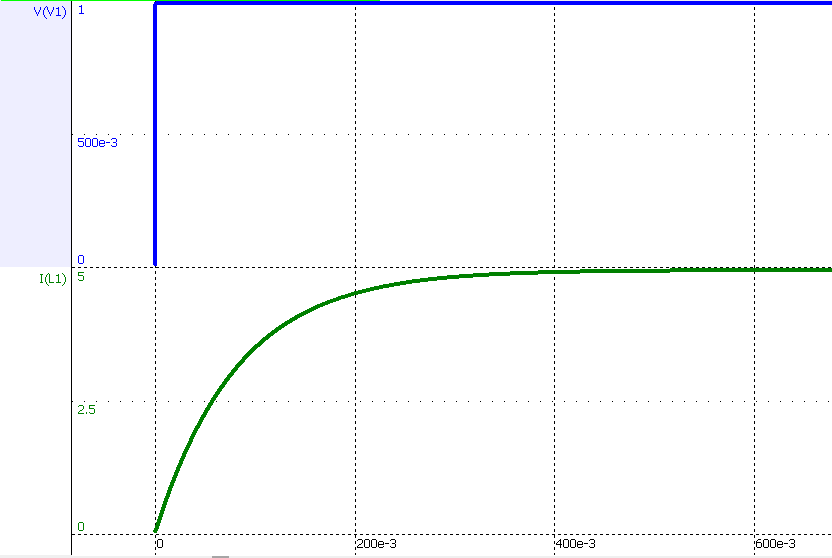
\includegraphics[scale=0.5]{corriente_escalon.png}
	\caption{Respuesta ante una entrada en escalón.}
	\label{fig:img_respuesta_escalon}
\end{figure}


\section{Diseño del controlador}

Se desea controlar el valor de la corriente que circula por el electroimán a partir de una tensión de referencia. Es decir, que la corriente sea proporcional a esta tensión de entrada. Para ello, se propone implementar un controlador que actúe sobre la tensión de alimentación del electroimán ($V_L$), ya que como dice la expresión \ref{eq_corriente}, esta permite modificar el valor de la corriente. Por lo tanto se propone el siguiente diagrama en bloques:


\begin{figure}[H]
	\centering
	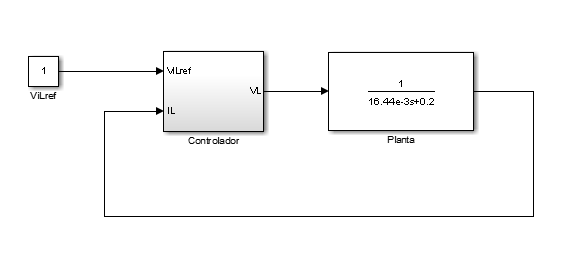
\includegraphics[scale=0.5]{Diagrama-en-bloques-basico.png}
	\caption{Diagrama en bloques básico.}
	\label{fig:img_diagrama_bloques_basico_cc}
\end{figure}

Este sistema de control trabaja a lazo cerrado, es decir, mide una tensión proporcional a la corriente y luego la compara con la referencia. Este resultado es utilizado para determinar si es necesario aumentar o disminuir la corriente y, en función de ello, actuar sobre la tensión de alimentación del electroimán.

Para ello se propone diseñar un controlador que trabaje en conmutación. En este tipo de controladores se alterna la alimentación del electroimán ($V_L$) entre un valor superior positivo $\ V_{sup}$, y un valor inferior negativo $V_{inf}$. De esta manera, al controlar los tiempos de conmutación, se logra que la corriente oscile en torno a un valor medio deseado. La forma de onda resultante se muestra en la figura  \ref{fig:img_corriente_exponencial}. En ella se puede ver que existe un ripple superpuesto al valor medio deseado. Sin embargo, esto no presentaría un problema si el controlador de corriente es diseñado de forma tal que estas variaciones sean pequeñas comparadas con el valor medio.

\begin{figure}[H]
	\centering
	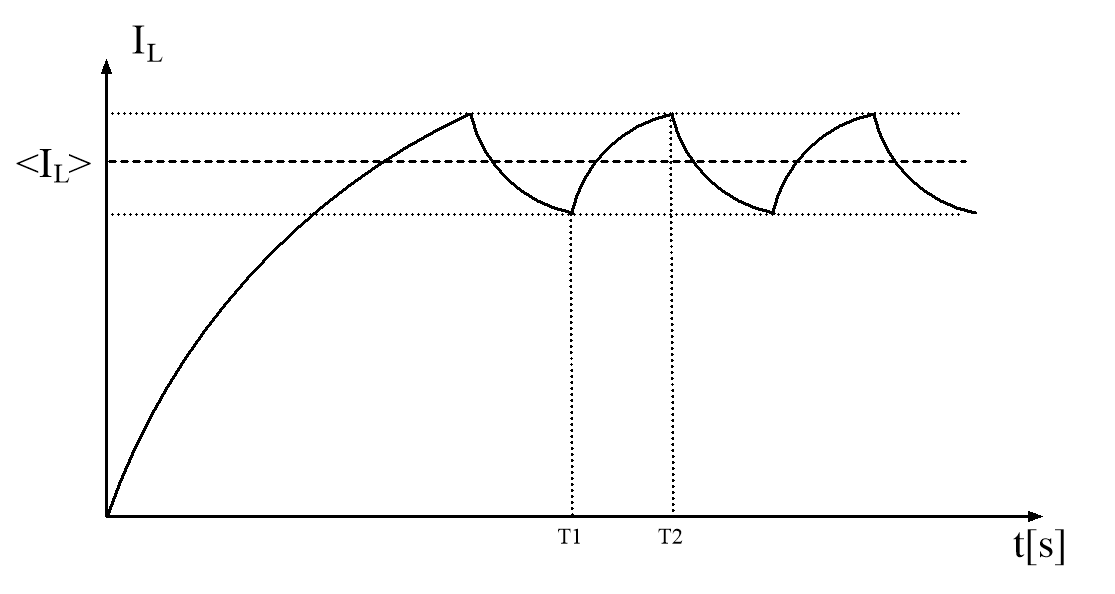
\includegraphics[scale=0.5]{Forma-de-onda-corriente-exponencial.png}
	\caption{Forma de onda de corriente y tensión en el electroimán.}
	\label{fig:img_corriente_exponencial}
\end{figure}

\colorbox{red}{modificar valores de imagen Vsup y Vinf}

Al elegir un período de conmutación lo suficientemente chico con respecto a la constante de tiempo de la planta, la forma de onda de la corriente en estado estacionario puede ser aproximada a una onda triangular como se muestra en la figura \ref{fig:img_corriente_lineal}. 

\begin{figure}[H]
	\centering
	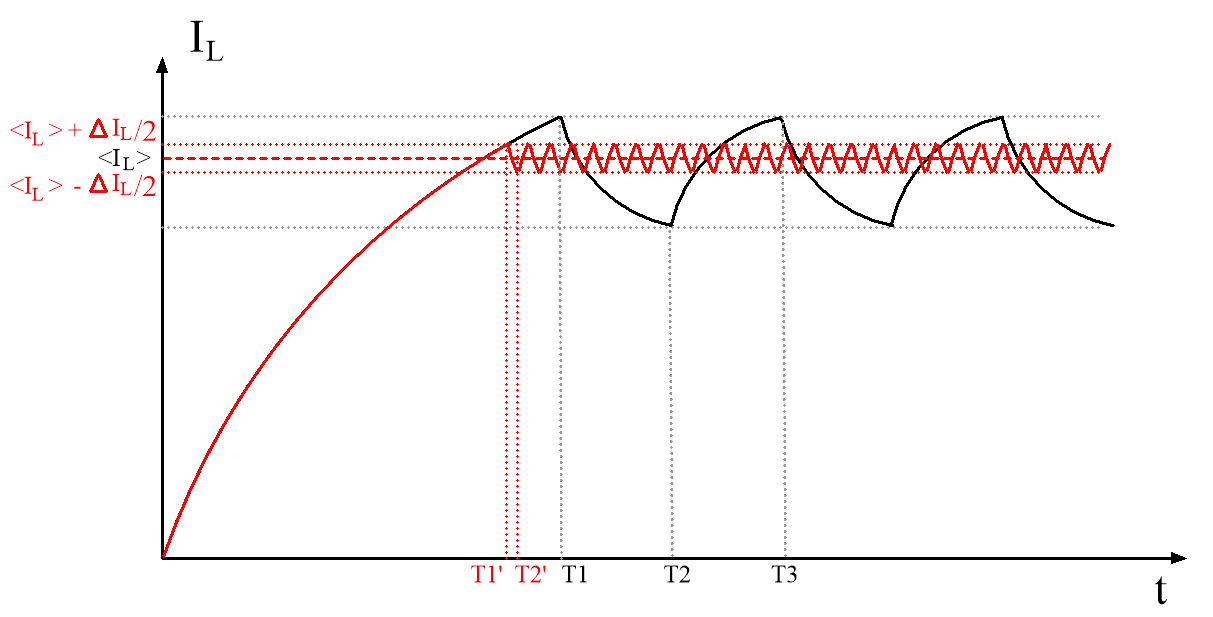
\includegraphics[scale=0.5]{Forma-de-onda-corriente-lineal.png}
	\caption{Forma de onda de corriente al disminuir el período de conmutación.}
	\label{fig:img_corriente_lineal}
\end{figure}

Cada tramo que compone la onda triangular puede ser aproximado con la ecuación \ref{eq_corriente_taylor}, en donde $I_o$ corresponde al valor de corriente en el que se produce la conmutación en $V_L$.

\begin{equation} \label{eq_corriente_taylor}
	i_L(t)=I_o -  (I_o-\frac{V_L}{R_L})*\frac{t}{\tau}
\end{equation}

Es posible observar en la expresión \ref{eq_corriente_taylor} que la pendiente de la onda triangular depende de $\tau=\frac{L_{(Y_g)}}{R_L}$. Es decir, se puede ver que existe una relación entre la pendiente y la distancia de entrehierro. Debido a que para poder determinar la magnitud de fuerza magnética que debe generar el electroimán es necesario conocer dicha distancia, se propone medirla indirectamente a través de la pendiente de la onda triangular. Por lo tanto, a continuación se analiza que variables del sistema afectan el valor de la pendiente y si es posible implementar el estimador de posición.

\subsection{Análisis de estimación de distancia de entrehierro}

Como se mencionó previamente, la pendiente de la onda triangular de la corriente contiene información de la distancia de entrehierro. Por lo tanto, para realizar este análisis se hace la derivada de la expresión \ref{eq_corriente_taylor} con respecto al tiempo para obtener el valor de la pendiente y se reemplaza $\tau=\frac{L_{(Y_g)}}{R_L}$.

%\begin{equation} \label{eq_derivada_corriente}
%	\frac{di_L(t)}{dt}=(\frac{V_L}{R_L}-I_o)*\frac{1}{\tau}
%\end{equation}

\begin{equation} \label{eq_derivada_corriente}
	\frac{di_L(t)}{dt}=\frac{V_L-I_o*R_L}{L_{(Y_g)}}
\end{equation}


Si bien la pendiente cambia según las condiciones iniciales, para este análisis se considera $I_o=0$ y luego se analizará cómo afecta en el sistema real. De esta forma, la pendiente resulta:


\begin{equation} 
	\frac{di_L(t)}{dt}= \frac{V_L}{L_{(Y_g)}}
\end{equation}


Como se vio en el capítulo \ref{cap:CaracterizacionElectroiman}, la expresión \ref{eq_inductancia_vs_y} indica que la inductancia del electroimán es inversamente proporcional a la distancia de entrehierro. Por lo tanto se llega a:

\begin{equation}\label{eq_pendiente_vs_Yg}
	\frac{di_L(t)}{dt}= Y_g*\frac{2}{N^2*A*\mu_o}*V_L
\end{equation}

En la expresión \ref{eq_pendiente_vs_Yg}, la tensión con la que se alimenta al electroimán está representada por $V_L$. A partir de la figura \ref{fig:img_corriente_lineal} se pueden plantear dos casos para la pendiente: cuando crece (con $V_L=V_{sup}$) y cuando decrece (con $V_L=V_{inf}$). Por lo tanto, se obtienen dos expresiones:

\begin{equation} 
	\frac{di_L(t)}{dt}_{sup}= Y_g*\frac{2}{N^2*A*\mu_o}*V_{sup}
\end{equation}


\begin{equation}
	\frac{di_L(t)}{dt}_{inf}= Y_g*\frac{2}{N^2*A*\mu_o}*V_{inf}
\end{equation}
%
%La tensión $V_L$ es un parámetro de diseño en el sistema, por lo tanto resulta conveniente elegir una fuente de alimentación para el electroimán que sea capaz de entregar una tensión, que llamaremos $V_{cc}$, alternando su polaridad. Por lo tanto $|V_{sup}|=|V_{inf}|=|V_{cc}|$. De esta forma, se obtiene que el módulo de la pendiente es igual en ambos casos y resulta:
%
%La tensión $V_L$ es un parámetro de diseño en el sistema, por lo tanto resulta conveniente elegir una alimentación $V_{cc}$ tal que $|V_{sup}|=|V_{inf}|=|V_{cc}|$. De esta forma, se obtiene que el módulo de la pendiente es igual en ambos casos y resulta:

Como se desea realizar la estimación a partir del módulo de la pendiente, resulta conveniente que su magnitud sea igual en cada ciclo de conmutación independientemente de la tensión de alimentación aplicada. Por lo tanto, debido a que la tensión $V_L$ es un parámetro de diseño en el sistema, se elijen valores de $V_{sup}$ y $V_{inf}$ que difieran en su polaridad, pero que tengan la misma magnitud. De esta forma, se define una alimentación $V_{cc}$ tal que $|V_{sup}|=|V_{inf}|=|V_{cc}|$ y se obtiene:
 
\begin{equation} \label{eq_pendiente_simetrica_corriente}
	\abs{\frac{di_L(t)}{dt}}= Y_g*\frac{2}{N^2*A*\mu_o}*\abs{V_{cc}}
\end{equation}

Como se muestra en la ecuación \ref{eq_pendiente_simetrica_corriente}, la pendiente varía únicamente con la distancia $Y_g$ puesto que los demás términos son constantes. 

De este análisis se llega a la conclusión de que es posible obtener una estimación de la distancia de entrehierro a partir de la medición de la pendiente de la onda triangular. Para ello se debe diseñar una fuente de alimentación que permita alternar la polaridad de la tensión aplicada al electroimán con igual magnitud pero sentido contrario.

\subsection{Lógica de control de corriente}

Para controlar la corriente que circula pr el electroimán y lograr la forma de onda triangular, se propone un controlador del tipo ON-OFF con el agregado de una zona de histéresis.

En la figura \ref{fig:img_diag-en-bloques} se puede observar el controlador implementado, en el cual la diferencia entre la corriente de referencia y la que circula por el electroimán está representada por $I_e$. Esta última ingresa al comparador con histéresis, que se encarga de alternar la polaridad de la tensión del electroimán según corresponda.

\begin{figure}[H]
	\centering
	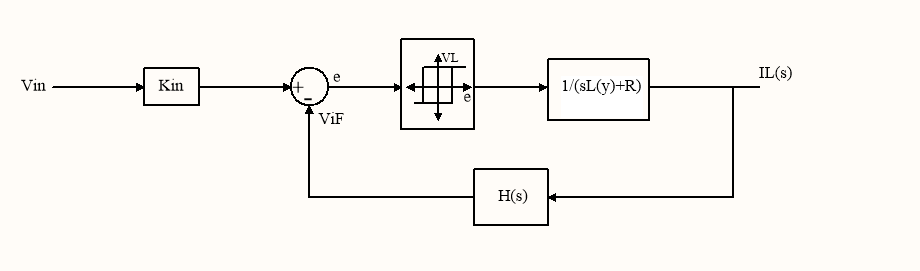
\includegraphics[width=\textwidth]{Diagrama-en-bloques.png}
	\caption{Diagrama en bloques del controlador de corriente con histéresis.}
	\label{fig:img_diag-en-bloques}
\end{figure}

\begin{figure}[ht]
	\centering
	%\begin{tikzpicture}[auto, node distance=2cm,>=latex']
%	\node [coordinate, name=entrada] {};
%	\node [sum, right=of entrada] (resta) {};
%	\node [coordinate, right=of resta] (ie) {};
%	\node [block, right=of ie] (comparador) {COMP};
%	\node [block, right=of comparador] (planta) {PLANTA};
%	\node [coordinate, right=of planta] (salida) {};
%	\node [coordinate, below of=planta] (realimentacion) {};
%	
%	\draw [->] (entrada) -- node {$I_{L_{ref}}$} (resta);
%	\draw [->] (resta) -- (comparador);
%	\draw [->] (comparador) -- (planta);
%%	\draw [->] (fft) -- node[name=a_resta] {} (resta);
%%	\draw [->] (fft) -- node[near end] {+} (resta);
%	\draw [->] (salida) |- (realimentacion);
%	\draw [->] (realimentacion) -| node[pos=0.95] {-} (resta);
%	\draw [->] (planta) -- node {$I_L$} (salida);
%	
%
%	
%%	\draw [->] (fft) |- (promedio);
%%	\draw [->] (promedio) -| node [near end] {-} (resta);
%\end{tikzpicture}

\tikzstyle{block} = [draw, fill=blue!20, rectangle, 
minimum height=3em, minimum width=6em]
\tikzstyle{sum} = [draw, fill=blue!20, circle, node distance=1cm]
\tikzstyle{input} = [coordinate]
\tikzstyle{output} = [coordinate]
\tikzstyle{pinstyle} = [pin edge={to-,thin,black}]

\def\windup{
	\tikz[remember picture,overlay]{
		\draw [stealth-stealth] (-1,0) -- node[pos=1] {$I_e$} (1,0); 
		\draw [stealth-stealth] (0,-0.6)--(0,0.6); %esto son los ejes
		\draw [-stealth] (-0.9,-0.4)-- (0.3,-0.4);
		\draw  [-stealth] (0.3,-0.4) -- (0.3,0.4); 
		\draw [-stealth] (0.9,0.4) --(-0.3,0.4);
		\draw [-stealth] (-0.3,0.4) -- (-0.3, -0.4); %esto sería la formita
}}
% The block diagram code is probably more verbose than necessary
\begin{tikzpicture}[auto, node distance=3cm,>=latex']
	% We start by placing the blocks
	\node [input, name=input] {};
	\node [sum, right of=input] (sum) {};
	\node [block, right of=sum] (controller) {\windup};
	\node [block, right of=controller, 
	node distance=3cm] (system) {System};
	% We draw an edge between the controller and system block to 
	% calculate the coordinate u. We need it to place the measurement block. 
	\draw [->] (controller) -- node[name=u] {$V_L$} (system);
	\node [output, right of=system] (output) {};
	\node [block, below of=u] (measurements) {Measurements};
	
	% Once the nodes are placed, connecting them is easy. 
	\draw [draw,->] (input) -- node {$I_{L_{ref}}$} (sum);
	\draw [->] (sum) -- node {$I_e$} (controller);
	\draw [->] (system) -- node [name=y] {$I_L$}(output);
	\draw [->] (y) |- (measurements);
	\draw [->] (measurements) -| node[pos=0.99] {$-$} 
	node [near end] {$I_{L_{feed}}$} (sum);
\end{tikzpicture}

	\caption{Diagrama en bloques simplificado del controlador de corriente}	\label{fig:diagrama_bloques_histeresis}
\end{figure}
\colorbox{red}{les parece? pueden modificarle cosas}

En este tipo de controlador se alterna la polaridad de la tensión de alimentación del electroimán, con el objetivo de que la corriente se mantenga oscilando en torno a un valor medio de referencia. Para ello se define un margen de corriente $\Delta I_L$ de forma tal que, si la corriente que circula por el electroimán supera a la de referencia, no se producirá un cambio de polaridad en la tensión aplicada hasta que la supere por $\frac{\Delta I_L}{2}$. Análogamente, cuando comienza a decrecer, seguirá haciéndolo hasta que sea menor a la corriente de referencia menos $\frac{\Delta I_L}{2}$.


Debido a que en las sucesivas conmutaciones lo único que cambia es la polaridad de la tensión con la que se excita al electroimán, la constante de tiempo del circuito no cambia. Esto da como resultado que la corriente oscile sobre un valor medio con igual tiempo de crecimiento que de decrecimiento. Esta oscilación también es conocida como \textsl{ripple}. Su amplitud es fija y está determinada por el ancho de histéresis con el que se diseñe el controlador.

Para lograr una forma de onda como la mostrada en la  figura \ref{fig:img_corriente_lineal} el controlador actúa de la siguiente manera. Al iniciar, la corriente $I_L$ es cero, dando como resultado a la entrada del comparador una $I_e = I_{ref}$. Por lo tanto, el comparador excita al electroimán con $V_L=+V_{CC}$ provocando que $I_L$ aumente de forma exponencial hasta que el valor de $I_e$ sea $\frac{\Delta I_L}{2}$. Una vez alcanzado este valor, el bloque con histéresis actúa y conmuta la tensión $V_L$ a $-V_{CC}$. Al hacer esto, la corriente comienza a decrecer hasta que el error sea igual a $-\frac{\Delta I_L}{2}$. De igual forma, en este punto el bloque comparador actúa y la tensión $V_L$ conmuta a $+V_{CC}$. Este ciclo se repite indefinidamente siempre y cuando la $I_{ref}$ sea constante. En caso de que esta cambie, el sistema dejará de conmutar momentáneamente hasta que el módulo de $I_e$ sea igual a $\frac{\Delta I_L}{2}$. Una vez igualado, el sistema volverá a conmutar.

TENEMOS QUE PONER LA IMAGEN Y CAMBIAR EL TEXTO EN REFERENCIA A ELLA

\subsection{Consideraciones prácticas del controlador de corriente}

En el diagrama en bloques \ref{fig:img_diag-en-bloques} se analizó la lógica de control trabajando únicamente con corrientes. Sin embargo, para la realización práctica del controlador es conveniente trabajar con tensiones. Por lo tanto, es necesario convertir el valor de corriente del electroimán medido en un valor de tensión proporcional, cuya ganancia se simboliza con $H(s)$ y esta determinado por el sensor a implementar. Por otro lado, para lograr que la corriente de salida excursione entre $0\:A$ a $30\:A$, a partir de una tensión de referencia de entrada, se agrega el bloque $K_{in}$ que permite relacionar cada valor de corriente de salida con uno de tensión de entrada. El diagrama en bloques del sistema modificado se muestra en la figura \ref{fig:img_diag-en-bloques-conH-y-Kin}.

\begin{figure}[H]
	\centering
	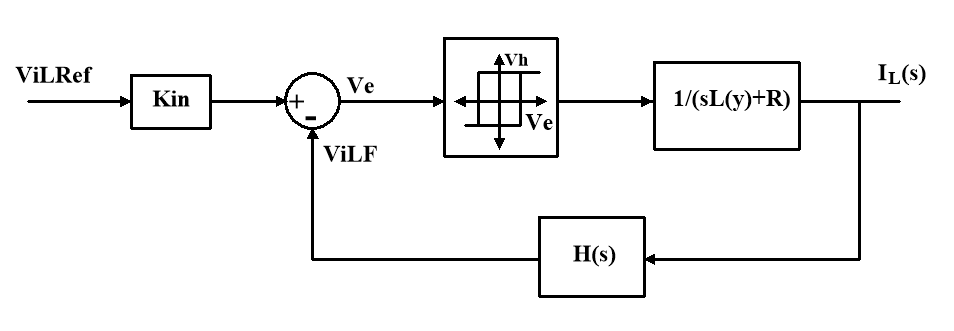
\includegraphics[width=\textwidth]{Diagrama-en-bloques-conH-y-Kin.png}
	\caption{Diagrama en bloques del controlador de corriente completo.}
	\label{fig:img_diag-en-bloques-conH-y-Kin}
\end{figure}

%Para hacer esto se debe utilizar un sensor que permita una medición de corriente hasta, por lo menos, $30\:A$  y con un error máximo tolerable tal que permita actuar al comparador y no afecte al sistema.

%ESTO AL FINAL ES AL PEDO CREO DE ULTIMA SE PUEDE HACER UN ANALISIS CON VALORES PERO MAS ADELANTE 
%Se puede expresar al error que introduce el sensor de efecto hall como $V_{errSensor}$. Entonces la expresión de error $V_{e}$ resulta: 

%\begin{equation}\label{eq_error_ve}
%	V_{e}= K_{in}*I_{ref}-H*iL\pm V_{errSensor}=\triangle I \pm V_{errSensor}
%\end{equation}


%De esta forma, tomando el  caso extremo $K_{in}*I_{ref}=H*i_{L}$ el error obtenido $V_{e}=\pm V_{errSensor}$.
%Es decir que el error es el propio error del sensor. Si se toma un ancho de histéresis mucho mayor al error máximo introducido por el sensor, este error no afectaría al sistema ya que seria despreciable a comparación del valor que deltaI debería alcanzar para que el comparador cambie de estado.

%El error que introduce el sensor de efecto hall $V_{errSensor}$ debe ser mucho menor al ancho de histéresis del comparador.

\subsection{Elección de topología de fuente de alimentación}

%La fuente de alimentación debe ser capaz de proveer la corriente que el eectroimán requiere para genera la fuerza suficiente para mantener al objeto en suspención. El sistema de control planteado en la sección anterior utiliza señales en forma de tensión, que tienen niveles bajos (son señales lñogicas)  Sin embargo el electroimán trabaja con corrientes de hasta 30 A, por lo tanto es necesario diseñar una etapa que haga la conversión entre señales de nivel lógico y señales de potencia.Por otro lado,
%
%Para poder controlar la corriente de hasta 30 A que circulan por el electroimán, se plantea utilziar una lógica de control con niveles de tensión entre 0V y 5V. 
%
%Para alcanzar los niveles de corriente de hasta 30A que requiere el electroimán es necesario implementar una etapa de potencia. Además, se debe tener en cuenta los siguientes aspectos. 

Para proveer la corriente que requiere el electroimán se decidió trabajar con una fuente conmutada. Debido a que existen diversas topologías circuitales para este tipo de fuentes, se analizan los aspectos que debe cumplir para poder elegir la adecuada.

Debido a que se medirá indirectamente la distancia de entrehierro a través de la pendiente de la onda triangular de la corriente, la topología debe permitir alternar la polaridad de la alimentación de forma tal que la magnitud de la pendiente se mantenga igual en cada semiciclo de conmutación. Es decir, la fuente debe ser capaz de alimentar al electroimán con $+V_{CC}$  en un semiciclo y con $-V_{CC}$ en el otro.

Por otro lado, debido a que el lazo de control para el sistema de levitación magnética necesitará conocer el valor de la distancia de separación de entrehierro para regular la fuerza ejercida, es necesario disponer de la estimación en todo momento. Por este motivo, no puede darse el caso en que el sistema deje de conmutar ya que no habría pendiente y, por ende, tampoco estimación de la distancia. Los casos en que la conmutación se podría ver afectada son los siguientes: 

\begin{itemize} 
	\item Cuando el sistema arranca desde corriente cero, hasta que el valor medio de corriente supera la mitad del ripple de corriente $(\Delta I_{L})$.
	
	\item Cuando la distancia de entrehierro es pequeña y se trabaja con peso reducido la corriente media puede llegar a ser menor que el ripple $\frac{\Delta I_{L}}{2}$.
\end{itemize}

Por estos motivos se propone utilizar una topología de puente H completo compuesto por cuatro llaves como se muestra en la figura \ref{fig:img_puente_h_con_llaves}.

\begin{figure}[H]
	\centering
	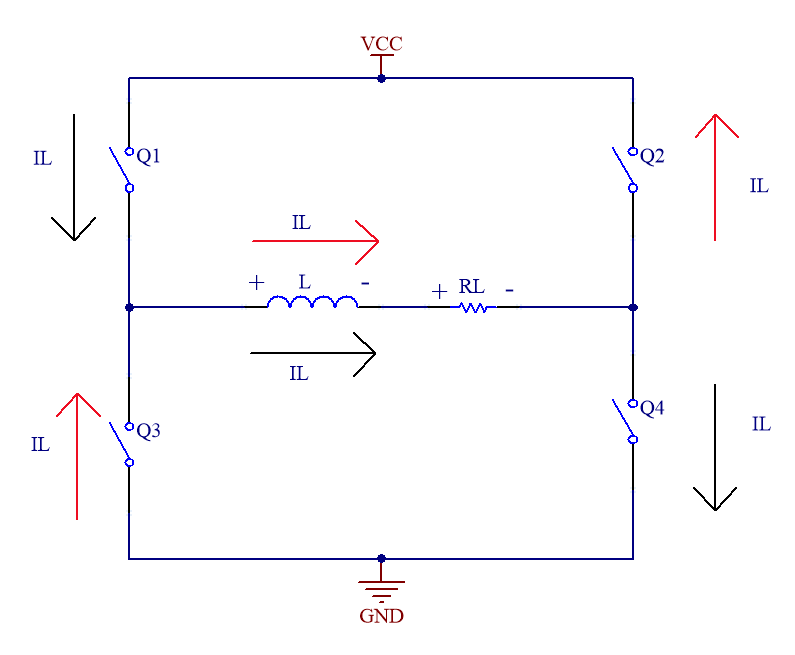
\includegraphics[width=\textwidth]{puente_con_llaves.png}
	\caption{Topología de puente H.}
	\label{fig:img_topologia_simplificada}
\end{figure}

\colorbox{pink}{poner un cuadrado en vez de la L y la R}

Esta topología permite el control individual del estado de cada llave. Cada una tiene dos estados posibles: abierto (no conduce corriente), y cerrado (conduce corriente sin caida de tensión en la llave). Por medio de la correcta combinación de llaves se puede lograr que la alimentación del electroimán sea $+V_{cc}$ (con Q1 y Q4 cerrados y Q2 y Q3 abiertos), o $-V_{cc}$ (con Q2 y Q3 cerrados y Q1 y Q4 abiertos). De esta manera, se logra una alimentación simétrica de la carga.

% Con estas combinaciones también se puede controlar el sentido de circulación de corriente.

Para esta aplicación en particular, la fuerza magnética es siempre en el mismo sentido, independientemente del sentido en que circule la corriente. Por lo tanto, se adopta como sentido de circulación positivo de izquierda a derecha como lo indican las flechas en la figura \ref{fig:img_topologia_simplificada}. 


% Esta topología permite la excursión negativa de la corriente mientras que mantiene en funcionamiento al estimador de posición.

\subsubsection{Funcionamiento del puente H}

Para poder obtener una forma de onda de corriente como la que se muestra en la figura \ref{fig:img_corriente_exponencial}, comenzando desde corriente nula, se debe controlar el estado de las llaves de la siguiente manera:


\begin{itemize}
	\item En principio se cierran las llaves $Q_1$ y $Q_4$ a la vez, generando un circuito entre $V_{CC}$, el electroimán y GND como indican las flechas negras en la figura \ref{fig:img_topologia_simplificada}. De esta forma, la corriente comienza a crecer con forma de exponencial negativa.
	\item Al llegar al límite superior de corriente ($I_{L_{MAX}}$), se debe conmutar el estado de las llaves, de manera que $Q_1$ y $Q_4$ dejen de conducir, y comiencen a hacerlo $Q_2$ y $Q_3$. De esta manera, la corriente seguirá circulando en el mismo sentido como indican las flechas rojas, pero ahora la diferencia de potencial en los bornes del electroimán se opone al paso de la corriente, por lo que su magnitud comienza a decrecer.
	\item Una vez alcanzado el límite inferior de corriente ($I_{L_{MIN}}$), se vuelve a conmutar el estado de las llaves para que la corriente vuelva a crecer.
	\item Este ciclo se repite en régimen permanente para que el valor medio de la corriente generada coincida con la deseada. 
\end{itemize}

Es importante tener en cuenta que sólo dos llaves pueden encenderse a la vez, y esto debe realizarse de manera diagonal. Es decir, en la figura \ref{fig:img_topologia_simplificada}, $Q_1$ y $Q_4$ pueden estar encendidos, mientras que $Q_3$ y $Q_2$ están apagados, y viceversa. Esto es debido a que se podría generar un cortocircuito entre la fuente de alimentación y GND, produciendo una circulación de corriente elevada que podría dañar el sistema y la fuente de alimentación. Se debe tener en cuenta esta restricción al momento de diseñar el circuito encargado de controlar estas llaves.

El valor de tensión de la fuente de alimentación utilizada para el puente H está basado en la versión anterior del dispositivo, por lo que se utiliza $V_{CC} = 24\:V$.

\section{Elección y cálculo de parámetros del controlador}

En esta sección se determinarán los parámetros críticos para el correcto funcionamiento del controlador de corriente.

%\subsection{Cálculo de tensión de alimentación}

%Como se esta excitando a un sistema RL que posee una constante de tiempo ($\tau$) definida con una conmutación de tensión $\pm Vcc$, la elección de este ultimo valor determina la velocidad de respuesta que el sistema tendrá ante perturbaciones o cambios en el punto  de operación.

%La determinación del valor de la tensión de alimentación $V_{CC}$ a utilizar es importante ya que determina la velocidad con la que responde el sistema ante perturbaciones o a cambios en el punto de operación. Por lo tanto, se analiza qué valor de tensión de alimentación es requerida para lograr aumentar la corriente que circula por el electroimán lo suficientemente rápido para que pueda responder ante esas situaciones.
%
%Para ello, se plantea el caso en que el sistema se encuentra con un objeto de 1Kg suspendido a una distancia de 5mm y este cambia abruptamente a 30Kg. 
% 
%Las condicion inicial del problema es un objeto de 1Kg suspendido a una distancia de 5mm, por lo que por el electroimán estarán circulando 3.72A. La condición final es una masa 30Kg a 6mm, lo que resulta en una corriente de 24.48A. Por lo tanto, el sistema debe ser lo suficientemente rapido para aumentar la corriente 20.75A antes de que el objeto llegue a 5mm. 
%
%Nos dio un Vcc de 26.79 (con una inductancia para 4mm)
%Nos dio un Vcc de 24.4 (con una inductancia para 5mm)
%Nos dio un Vcc de 23.7 (con una inductancia para 6mm)
%\colorbox{red}{repetir cálculo con y=4}
%\begin{equation}
%	I_L(Y=4\:mm)[m=1\:kg]=3.72\:A  
%\end{equation}
%
%\begin{equation}
%	I_L(Y=5\:mm)[m=30\:Kg]=20.4\:A 
%\end{equation}
%
%Antes de llegar a un tiempo....T1
%%Es importante determinar cómo será la alimentación del controlador de corriente. Para hacerlo se debe tener en cuenta la velocidad de respuesta de la planta que está determinada por su constante de tiempo ($\tau$). Es decir, el sistema debe ser lo suficientemente rápido para modificar el valor medio de la corriente ante perturbaciones o cambios en el punto de operación. 
%
%
%
%Un caso a analizar es cuando, en régimen permanente, se modifica bruscamente la carga que esta levitando. En esta situación el sistema debe aumentar o disminuir la corriente de forma abrupta para evitar que el objeto se caiga. El caso de mayor exigencia se da cuando a una distancia máxima de referencia $Y_g=5\:mm$ se modifica de carga mínima ($1\:Kg$) a máxima ($30\:Kg$). Utilizando la ecuación \label{eq_corriente_peso} se obtiene que la corriente para ambos casos es de:
%
%Es importante tener en cuenta que la inductancia se consideró constante.
%
%
%
%
%Dado que el polo dominante ya está definido por el circuito RL del electroimán, la velocidad con que el sistema pueda alcanzar un valor de corriente elevado está determinado por el valor de la fuente de alimentación. La expresión teórica de la corriente es: 
%
%\begin{equation}
%	I_L(t)=\frac{V}{R_L} + (I_o-\frac{V}{R_L})*e^{-\frac{t}{\tau}}
%\end{equation}
%
%Donde:
%\begin{itemize}
%	\item V es la tensión de alimentación, que puede tomar valores $+V_{cc}$ y $-V_{cc}$.
%	\item $I_o$ es la corriente en el instante inicial.
%	\item $\tau$ es la constante de tiempo del electroimán.
%\end{itemize}
%
%Para encontrar la expresión del tiempo que tarda la corriente en alcanzar el valor máximo de corriente $i_{max}$ se reemplaza $I_{0}=2.9$ y se obtiene $T_{1}$. Esto da:
%
%\begin{equation}\label{eq_tiempo_de_subida}
%	T_1=-\tau*ln(\frac{V_{cc}-R*I_{max}}{V_{cc}-R*I_{0}})
%\end{equation}
%
%Cuando se modifique la carga del objeto ,es necesario que el tiempo de subida de corriente $T_1$ sea mucho menor al tiempo en que la carga llegue a la distancia máxima que el sistema soporta $Y=5mm$ aprox (que corresponde a $I_{max}$). Es decir que el objeto cae libremente un delta $\Delta Y= 1mm $. Utilizando la ecuación \ref{eq_caida_libre} se obtiene el tiempo (T) que tarda en desplazarse un objeto en caída libre una altura $\Delta Y$:
%
%\begin{equation}\label{eq_caida_libre}
%	T=\sqrt{\frac{2*\Delta Y}{g}}=\sqrt{\frac{2*1mm}{9.81}}=14,27\:ms
%\end{equation}
%
%Reemplazando este valor en la ecuación \ref{eq_tiempo_de_subida} se puede obtener el valor de tensión mínimo de $V_{CC}$ para que se alcance una velocidad de respuesta aceptable para que circule la corriente necesaria para que el objeto mantenga la posición deseada.
%
%El valor obtenido es $Vcc\geq21.6\:V$ por lo que se escoge un valor comúnmente utilizado de $24 V$.
%
%
%colorbox{Se puede decir cuanto da $T_1$ si tomamos 24V.}

\subsection{Cálculo de ancho de histéresis}

%Como se mencionó, se desea controlar la fuerza ejercida a partir del valor medio de la corriente. Por lo tanto, las variaciones en torno a dicho valor medio no deben generar variaciones significativas en la fuerza magnética. Por ello, se debe elegir un ancho de histéresis tal que la frecuencia de conmutación resultante sea filtrada por la dinámica de la planta. Un valor de al menos 100 veces mayor que la frecuencia del polo de la planta obtenida en \ref{eq_transferencia_planta_m} serìa suficiente. Este se ubica en $70\:r/s$, lo que resulta en que se debe conmutar a una frecuencia de $\omega_{sw}>=7000\:r/s$, y expresada en Hz resulta $F_{sw}>=1\:kHz$.

Para controlar la fuerza magnética ejercida sin tener variaciones los componentes frecuenciales introducidos por la conmutación deben ser filtrados por la dinámica de la planta.

Esto se logra asignando una frecuencia de conmutación con un valor de al menos 100 veces mayor que la frecuencia del polo de la planta obtenida en \ref{eq_transferencia_planta_m}.
De esta forma el polo dominante se mantiene y la respuesta a los transitorios no se ve afectada.  Este se ubica en $70\:r/s$, lo que resulta en que se debe conmutar a una frecuencia de $\omega_{sw}\geq7000\:r/s$ (expresada en Hz resulta $F_{sw}\geq1\:kHz$).


Por lo tanto, como la frecuencia mínima es $F_{sw}$, y considerando que el tiempo en que crece la corriente es igual al que decrece, se obtiene que el tiempo máximo que puede tener la sección creciente de la corriente es igual a $t_{max}=500\:us$. 

A partir de la expresión \ref{eq_corriente_temporal_cond_iniciales} se puede obtener el valor máximo de ripple cuando $t=t_{max}$, considerando que la corriente inicial es $I_{min}$ y que la corriente final es $I_{min}+\Delta I_L$

\begin{equation} \label{eq_delta_i}
	I_{min}+\Delta I_{L_{max}}=\frac{V_{CC}}{R_L}+(I_{min}-\frac{V_{CC}}{R_L})*e^{-\frac{t_{max}}{\tau}}
\end{equation}

De la ecuación \ref{eq_delta_i} se obtiene el valor máximo que se le puede asignar a $\Delta I_L$. 

\begin{equation} \label{eq_delta_i_2}
	\Delta I_{L_{max}}=6.06*10^{-3}*(\frac{V_{CC}}{R_L}-I_{min})
\end{equation}
\colorbox{red}{ver imagen de altium}

El controlador de corriente tendrá una corriente media variable entre 0 y 30 A, se debe satisfacer la expresión \ref{eq_delta_i_2} para cualquier $I_{min}$ dentro de ese rango. Por lo tanto se plantean dos casos: $I_{min}=0$ e $I_{min}=30$. Para el primer caso se obtiene que $\Delta I_{L_{max}}=727\:mA$ y en el segundo $\Delta I_{L_{max}}=500\:mA$. Por lo tanto se elige un ancho de histéresis de $500\:mA$ ya que cumple las dos condiciones.

\subsection{Elección del sensor de corriente}

Como se menciono en secciones anteriores es necesario realizar una medición sobre la corriente que circula por el bobinado del electroimán para que luego el controlador pueda actuar en consecuencia. Es necesario conocer tanto su valor medio, como su ripple. Es por ello que se debe idear una estrategia de medición que represente correctamente esta forma de onda cuyo valor medio puede alcanzar valores desde 0 hasta 30 A con un ripple de 500 mA.

En esta sección se analizan dos alternativas para lograr este objetivo. La primera mediante una resistencia en serie al electroimán y la segunda utilizando un sensor de efecto Hall.


\subsubsection{Análisis de medición de corriente mediante resistencia shunt}
La forma de medir corriente que resulta, en principio, más simple es la de utilizar una resistencia de valor $R_s$ en serie con el electroimán como se muestra en la figura \ref{fig:img_puente_con_rshunt}, y medir en sus terminales la diferencia de tensión generada por la corriente. A partir de esta tensión ($V_s-V_a$) se puede utilizar la ley de Ohm para conocer el valor de corriente:

\begin{equation}
	I_L=\frac{V_s-V_a}{R_s}
\end{equation}


\begin{figure}[H]
	\centering
	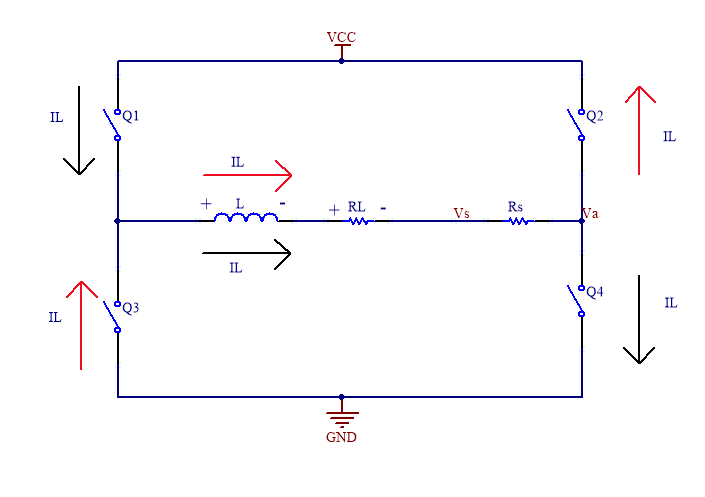
\includegraphics[width=\textwidth]{puente_con_rshunt.png}
	\caption{Puente H con resistencia de sensado de corriente (Rs).}
	\label{fig:img_puente_con_rshunt}
\end{figure}

Por otro lado, la realimentación del controlador de corriente debe ser en forma de tensión, por lo tanto es suficiente con medir la tensión diferencial $V_s-V_a$ y tener en cuenta en el diseño del controlador la ganancia que se tiene al pasar de corriente a tensión.

Aunque este método para medir corriente pareciera directo, presenta algunos inconvenientes en el diseño:

El primero es que al agregar una resistencia en serie al electroimán, se introduce una mayor disipación de potencia en el sistema. Para intentar reducir este problema se podría elegir un valor de resistencia lo suficientemente bajo para que su consumo sea despreciable. Por ejemplo, si se adopta una resistencia de $10\:mOhms$ el valor de pérdidas de potencia es de $4\:W$, que es un valor aceptable. 

El segundo inconveniente es que se altera la dinámica de la planta, ya que la constante de tiempo cambia a $\tau=\frac{L}{R_L+R_s}$. Sin embargo, el electroimán presenta una resistencia interna de $0.2\:Ohm$, por lo que una resistencia de sensado con valor $10\:mOhm$ no afectaría en gran medida la dinámica.

El tercero es que se debe realizar una medición de tensión flotante. Esto se debe a que la resistencia, al estar en serie con el electroimán, no tiene ningún punto de medición referido a masa. Por lo tanto, se debe utilizar un amplificador que mida tensión en modo diferencial para luego obtener una señal en modo común. El inconveniente que se presenta es que cada uno de los puntos de medición se encuentra a un alto potencial respecto de masa y, además, este cambia en cada conmutación. Esto genera que durante los transitorios de conmutación haya ruido en la medición diferencial.

Debido a que se requiere medir el valor de corriente sin que el ruido de modo común altere la medición, se propone analizar otra alternativa que sea inmune a dicho efecto.


\subsubsection{Análisis de medición de corriente mediante sensor de efecto Hall}

Dado que la medición con una resistencia de shunt introduce ruido ocasionado por la conmutación de las llaves, se plantea como alternativa utilizar un sensor de efecto Hall. Estos dispositivos miden el campo magnético generado por la corriente, entregando a su salida una tensión proporcional a ésta. La principal ventaja que presentan es que el campo magnético medido sólo es sensible a las variaciones de corriente y no a las conmutaciones de tensión.

Existen una gran variedad de estos sensores en el mercado, cada uno con diferentes características. A continuación se mencionan los criterios que se tendrán en cuenta para la elección del sensor:

\begin{itemize}
	\item Debe ser capaz de medir una corriente de hasta $30\:A$.
	\item El ancho de banda debe ser mucho mayor al polo de la frecuencia de conmutación del controlador de corriente para poder conservar la forma de onda de la corriente triangular a medir. Por lo tanto, debe ser al menos de $100\:kHz$.
	\item La transresistencia debe ser lineal entre $0\:A$ y $30\:A$.	
\end{itemize}

A partir de estas características se decidió utilizar el sensor HO 15-NP-0000 \cite{HO15-NP}. Este permite medir una corriente de $\pm 37.5\:A$ con un ancho de banda de $250\:kHz$ y posee una transresistencia de $53.33\:mV/A$ en todo  el rango de corriente. Además, presenta alta inmunidad a interferencias externas. 

Este sensor tiene la capacidad de medir tanto corrientes en sentido positivo, como negativo. Para ello admite una tensión de bias de $2.5\:V$, la cual se corresponde a la salida cuando la corriente es nula. Cuando la circulación de corriente es positiva, la salida del sensor resulta en una tensión mayor a $2.5\:V$, y para negativas, menor.

De esta forma, el bloque H de realimentación queda definido como:

\begin{equation}
	H=\frac{V_iLF}{I_L}=53,33 mV/A
\end{equation}



\subsection{Cálculo de ganancia de entrada}


